\section{Experiments}
\label{sec:experiments}

We evaluate the currently implemented components of the framework under a controlled within-mine setting. The experiments address four questions: 1) whether repeated human driving provides a useful trajectory prior on a held-out traversal; 2) whether an imitation policy that performs well under open-loop evaluation remains stable under recursive closed-loop execution; 3) whether action-conditioned risk screening reduces boundary violations; and 4) whether camera--LiDAR-derived vehicle motion can support collision-aware candidate selection. Reinforcement learning and physical deployment are outside the scope of the reported results.

\subsection{Experimental Setup}
\label{sec:experimental_setup}

\subsubsection{Dataset and data separation}

The dataset contains seven repeated human-driven traversals, M0S0--M0S3 and M0S5--M0S7, collected in the same operational open-pit mine. The acquisition platform carries six synchronized cameras, a 64-beam Ouster LiDAR, and a GNSS/RTK-aided odometry system. The LiDAR measurements are expressed in the vehicle base frame, which is also the odometry child frame. Accurate poses provide trajectory-level supervision without requiring recorded steering, throttle, or braking commands.

Training, validation, and test data are separated by complete traversal rather than by individual frames. M0S0, M0S1, M0S2, M0S3, and M0S5 are used for training, M0S6 for validation, and M0S7 only for testing. Temporally adjacent samples from one traversal therefore never appear in different splits. Because all traversals come from one mine, the evaluation measures within-mine, cross-traversal generalization and does not establish cross-mine or long-term generalization.

\subsubsection{Imitation-learning protocol}

Samples are selected at $0.5\,\mathrm{Hz}$ to reduce temporal correlation, producing 1,705 training, 378 validation, and 304 test samples. Each sample contains a five-channel LiDAR bird's-eye-view (BEV) representation over an $80\times80\,\mathrm{m}$ region at $0.5\,\mathrm{m}$ resolution, the current vehicle state $[v_x,v_y,\dot{\psi}]$, and a local goal obtained from the pose 8\,s in the future. The BEV channels encode mean height, height variance, point density, vertical-span obstacle evidence, and an observation mask. Expert waypoints at 1--5\,s are generated from future odometry poses and expressed in the current vehicle frame.

The policy predicts the mean and log standard deviation of five local waypoints and is trained for 60 epochs using Gaussian trajectory negative log-likelihood. Model selection uses only M0S6. For closed-loop evaluation, BEVs are rendered from reconstructed training-session point maps at the recorded expert poses, matching the observation process used by the simulator. The held-out M0S7 map is used only to render test observations and is never used for parameter optimization or model selection. The reported learning results use one random seed.

\subsubsection{Closed-loop simulator}

We construct a lightweight data-driven simulator from the reconstructed point maps and expert routes. At each simulated pose, the global point map is cropped, transformed into the current vehicle frame, and rasterized using the same five-channel BEV representation used during training. Vehicle motion follows a kinematic bicycle model with a $4.5\,\mathrm{m}$ wheelbase and a $3.5\,\mathrm{m}$ vehicle width. A Pure Pursuit controller executes the selected trajectory at 10\,Hz, while the policy replans at 2\,Hz. The boundary-recovery evaluation uses a fixed task speed of $5\,\mathrm{m\,s^{-1}}$ to isolate lateral stability. The dynamic-replay evaluation additionally permits target speeds of 0, 1, 2.5, and $5\,\mathrm{m\,s^{-1}}$.

Each episode covers a 120\,m route segment. Ten route starting locations are combined with nominal initialization, lateral offsets of $\pm1$, $\pm2$, and $\pm3\,\mathrm{m}$, and heading offsets of $\pm5^\circ$, $\pm10^\circ$, and $\pm15^\circ$, giving 130 episodes per method. A run succeeds if the vehicle completes the segment without its footprint leaving the estimated 12\,m transportation corridor. A perturbed run is counted as recovered if its lateral error remains below 1\,m and its heading error remains below $5^\circ$ for at least 2\,s.

The simulator is intended for controlled algorithm validation. The road width, vehicle dimensions, and kinematic response are approximations. The boundary experiments contain no inserted traffic. A separate dynamic-replay experiment introduces moving vehicles using motion statistics extracted from the recorded traversals; it does not model pedestrians or high-fidelity vehicle interaction.

\subsection{Open-Loop Imitation Initialization}
\label{sec:open_loop_il}

We first test whether repeated driving provides a useful trajectory prior. The learned policy is compared with constant-velocity extrapolation and linear interpolation from the current pose toward the 8\,s local goal. Average displacement error (ADE) measures the mean error over the 1--5\,s horizon, while final displacement error (FDE) measures the endpoint error at 5\,s.

\begin{table}[t]
\centering
\caption{Open-loop trajectory prediction on 304 held-out M0S7 samples.}
\label{tab:il_trajectory_prediction}
\resizebox{\columnwidth}{!}{%
\begin{tabular}{lccc}
\toprule
Method & ADE (m) $\downarrow$ & FDE (m) $\downarrow$ & P95 FDE (m) $\downarrow$ \\
\midrule
Constant velocity & 1.430 & 3.146 & 8.841 \\
Linear to local goal & 1.537 & 1.787 & 5.142 \\
Imitation policy & \textbf{0.944} & \textbf{1.195} & \textbf{3.192} \\
\bottomrule
\end{tabular}}
\end{table}

The imitation policy reduces ADE by 34.0\% and 5\,s FDE by 62.0\% relative to constant-velocity extrapolation. Its mean displacement errors at 1, 2, 3, 4, and 5\,s are 0.438, 0.797, 1.076, 1.216, and 1.195\,m, respectively. It also outperforms direct interpolation toward the local goal, indicating that it captures trajectory structure beyond current velocity and goal direction. These results support its use as an initialization policy but do not establish closed-loop stability.

Figure~\ref{fig:il_qualitative} visualizes representative predictions on M0S7. The policy follows the demonstrated direction and curvature, although the sample-dependent displacement errors indicate that small open-loop deviations can remain.

\begin{figure*}[t]
\centering
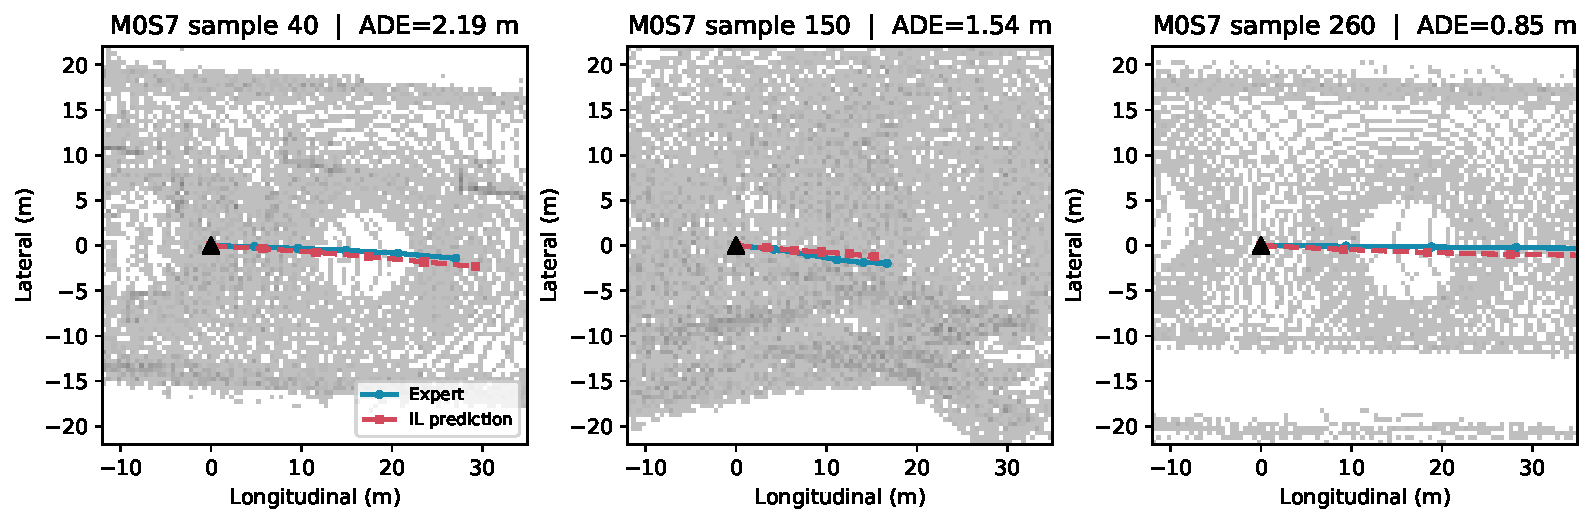
\includegraphics[width=0.96\textwidth]{figures/il_qualitative_m0s7.pdf}
\caption{Qualitative trajectory prediction on held-out M0S7 samples. The LiDAR BEV is shown in gray; blue and red denote the expert and imitation-policy trajectories, respectively.}
\label{fig:il_qualitative}
\end{figure*}

\subsection{IL-Only Closed-Loop Evaluation}
\label{sec:il_closed_loop}

We next execute the imitation predictions recursively. The policy receives observations generated from its current simulated pose, and its state is never reset to the expert trajectory. Despite its open-loop accuracy, the IL-only policy completes only 1.54\% of the 130 episodes and violates the corridor boundary in 98.46\%. It travels 59.52\,m on average before termination, and none of the perturbed episodes meets the recovery criterion. This gap demonstrates covariate shift: small prediction errors move the vehicle away from the expert-state distribution, after which errors accumulate.

To verify that the failure is not caused solely by the vehicle model or boundary definition, we run a privileged reference-route controller using the same initial states, dynamics, speed, and termination criteria. It completes all 130 episodes, with a mean lateral error of 0.566\,m. This controller is reported only as a simulator-validity upper bound because it directly accesses the held-out route.

\subsection{Action-Conditioned Boundary Risk}
\label{sec:risk_experiments}

We first evaluate terrain-boundary violation independently of dynamic traffic. Collision risk is evaluated separately using the dynamic-replay protocol below.

For each reconstructed training-session map, we sample expert-route states with lateral offsets of $-3$, 0, and $3\,\mathrm{m}$ and heading offsets of $-10^\circ$, 0, and $10^\circ$. At each state, 25 candidate trajectories combine five heading variations, $\{-15^\circ,-7.5^\circ,0^\circ,7.5^\circ,15^\circ\}$, with five terminal lateral offsets, $\{-3,-1.5,0,1.5,3\}\,\mathrm{m}$. Boundary labels are computed from the candidate's swept vehicle footprint and the estimated transportation corridor.

M0S0, M0S1, M0S2, M0S3, and M0S5 provide 45,000 training observation--trajectory pairs. M0S6 provides 9,000 validation pairs, and M0S7 provides 9,000 test pairs. The positive boundary-risk rate on M0S7 is 43.2\%. The risk model receives the BEV, vehicle state, local goal, and candidate trajectory; it does not receive the ground-truth boundary label or privileged collision state.

\begin{table}[t]
\centering
\caption{Boundary-risk prediction on 9,000 held-out M0S7 observation--trajectory pairs.}
\label{tab:risk_prediction}
\resizebox{\columnwidth}{!}{%
\begin{tabular}{lcccc}
\toprule
Model & AUROC $\uparrow$ & AUPRC $\uparrow$ & Brier $\downarrow$ & ECE $\downarrow$ \\
\midrule
Action-conditioned risk model & 0.943 & 0.937 & 0.102 & 0.070 \\
\bottomrule
\end{tabular}}
\end{table}

The risk model achieves an AUROC of 0.943 and an AUPRC of 0.937 on the held-out traversal. The Brier score of 0.102 and ten-bin expected calibration error of 0.070 indicate useful, though imperfect, calibration across the evaluated candidate distribution.

Figure~\ref{fig:boundary_candidates} shows that the model assigns different risks to actions evaluated from the same observation. Candidates directed toward the unsafe side of the estimated corridor receive high probability, whereas candidates remaining in the feasible region receive low probability. The highlighted curve is the candidate with the lowest predicted boundary risk; closed-loop selection additionally accounts for deviation from the IL proposal.

\begin{figure}[t]
\centering
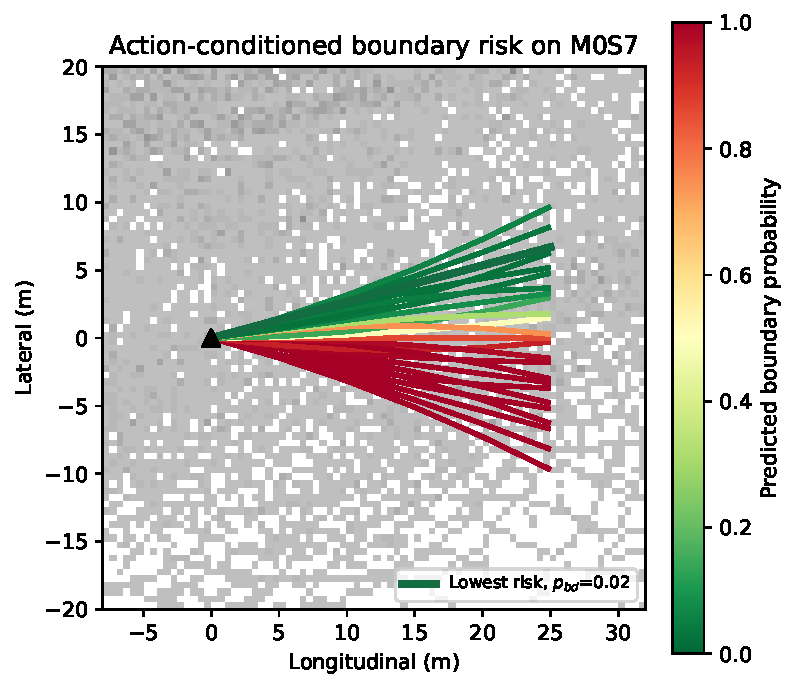
\includegraphics[width=0.95\columnwidth]{figures/boundary_candidate_screening.pdf}
\caption{Action-conditioned boundary-risk predictions for 25 candidate trajectories on M0S7. Color denotes predicted boundary probability, and the highlighted curve has the lowest predicted risk.}
\label{fig:boundary_candidates}
\end{figure}

\subsection{Dynamic-Actor Extraction and Collision Prediction}
\label{sec:collision_prediction}

We detect vehicles in all six camera streams and associate each detection with synchronized LiDAR points using the calibrated camera--LiDAR transforms. LiDAR-supported detections are transformed to the map frame using odometry and linked across time. Tracks shorter than 2\,s, faster than $15\,\mathrm{m\,s^{-1}}$, or classified as stationary are excluded. This automatic procedure yields 147 training tracks from M0S0, M0S1, M0S2, M0S3, and M0S5, 24 validation tracks from M0S6, and five test tracks from M0S7.

The collision model jointly encodes a candidate ego trajectory and the predicted five-second actor trajectory. Candidate actions combine three heading variations, five terminal lateral offsets, and target speeds of 0, 1, 2.5, and $5\,\mathrm{m\,s^{-1}}$, producing 60 trajectory candidates. Measured target speeds and motion directions are retained, while relative position and arrival time are randomized to construct controlled interactions. The resulting dataset contains 846,720 training, 138,240 validation, and 28,800 test trajectory pairs. These pairs are replay augmentations derived from 176 source tracks rather than independent observed encounters.

\begin{table}[t]
\centering
\caption{Action-conditioned collision prediction on 28,800 M0S7 replay pairs. Results are mean $\pm$ standard deviation over three training seeds.}
\label{tab:collision_prediction}
\resizebox{\columnwidth}{!}{%
\begin{tabular}{lcccc}
\toprule
Model & AUROC $\uparrow$ & AUPRC $\uparrow$ & Brier $\downarrow$ & ECE $\downarrow$ \\
\midrule
Collision-risk model & $0.99795\!\pm\!0.00008$ & $0.99270\!\pm\!0.00027$ & $0.02010\!\pm\!0.00091$ & $0.02335\!\pm\!0.00183$ \\
\bottomrule
\end{tabular}}
\end{table}

The high ranking accuracy shows that the model learns candidate--actor collision geometry under the replay distribution. It does not constitute an end-to-end perception result because tracked actor motion is supplied explicitly to the collision head.

Figure~\ref{fig:collision_candidates} illustrates the action-dependent output for one held-out replay interaction. Candidates whose future envelopes approach the tracked actor receive high collision probabilities, while alternative lateral or longitudinal responses remain low risk. The highlighted trajectory is the lowest-risk candidate before applying the boundary, imitation-deviation, and delay terms used by the complete selector.

\begin{figure}[t]
\centering
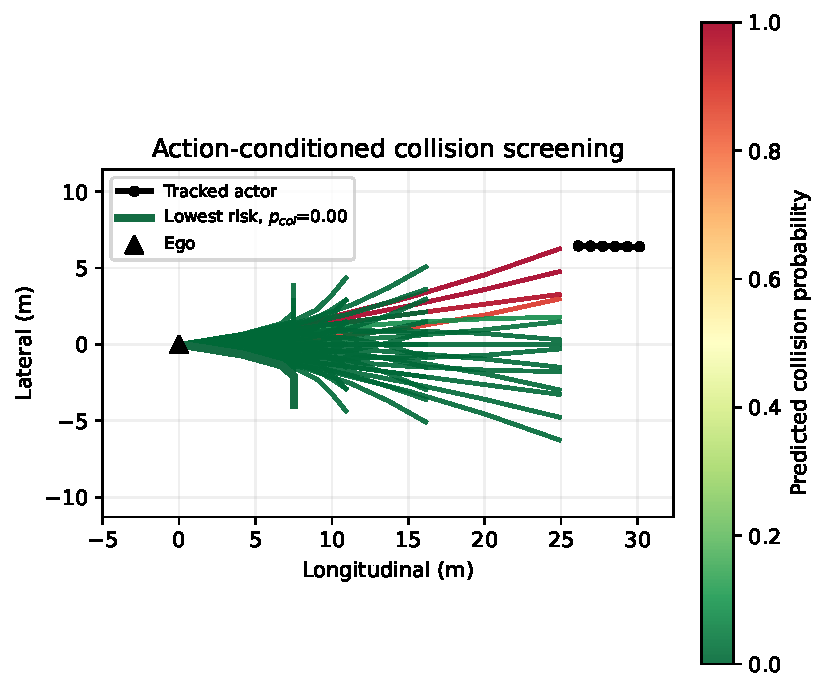
\includegraphics[width=0.95\columnwidth]{figures/collision_candidate_screening.pdf}
\caption{Collision-risk predictions for 60 longitudinal and lateral candidates in a held-out replay interaction. The black trajectory denotes the tracked actor, and the highlighted curve has the lowest predicted collision risk.}
\label{fig:collision_candidates}
\end{figure}

\subsection{Risk-Screened Closed-Loop Navigation}
\label{sec:risk_screened_navigation}

At each planning step, the IL policy produces a reference trajectory, and the risk module evaluates all 25 candidates. Candidate selection minimizes predicted boundary risk plus a penalty for deviation from the IL trajectory, with $\lambda_D=0.02$. The value is fixed without using M0S7 outcomes. No policy parameters are updated in this experiment, so the comparison isolates the effect of action-conditioned risk screening.

\begin{table}[t]
\centering
\caption{Closed-loop comparison on the same 130 M0S7 episodes. Values for success, boundary violation, and recovery are percentages. The privileged route controller is a simulator-validity upper bound.}
\label{tab:closed_loop}
\resizebox{\columnwidth}{!}{%
\begin{tabular}{lccccc}
\toprule
Method & Success $\uparrow$ & Boundary $\downarrow$ & Recovery $\uparrow$ & Lat. error (m) $\downarrow$ & Progress (m) $\uparrow$ \\
\midrule
IL only & 1.54 & 98.46 & 0.00 & 2.444 & 59.52 \\
IL + risk screening & \textbf{89.23} & \textbf{10.77} & \textbf{43.33} & \textbf{1.345} & \textbf{114.23} \\
Privileged route upper bound & 100.00 & 0.00 & 100.00 & 0.566 & 120.00 \\
\bottomrule
\end{tabular}}
\end{table}

Risk screening increases success from 1.54\% to 89.23\% and reduces boundary violations from 98.46\% to 10.77\%. Mean progress increases from 59.52 to 114.23\,m, while mean lateral error decreases from 2.444 to 1.345\,m. Recovery remains more difficult than nominal completion: 43.33\% of perturbed episodes satisfy the strict recovery criterion. These results show that candidate-level boundary prediction can mitigate imitation covariate shift without updating the base policy.

The comparison establishes boundary recovery under a fixed candidate family but does not by itself evaluate dynamic collision avoidance. We therefore perform the following controlled replay experiment.

\subsection{Dynamic-Replay Closed-Loop Evaluation}
\label{sec:dynamic_closed_loop}

We construct 150 M0S7 episodes from ten route starts, five held-out target-motion tracks, and following, opposing, and stopped-vehicle interactions. All methods use the same IL proposal and boundary-risk model. The emergency-braking baseline selects a stopping candidate when a constant-motion check predicts collision. Geometric checking evaluates the swept vehicle envelopes analytically, whereas learned screening first rejects candidates whose predicted collision probability exceeds 0.7 and then minimizes boundary risk, IL deviation, and delay. The threshold is selected on M0S6 and fixed for M0S7.

\begin{table}[t]
\centering
\caption{Controlled dynamic-replay closed-loop results on 150 M0S7 episodes.}
\label{tab:dynamic_closed_loop}
\resizebox{\columnwidth}{!}{%
\begin{tabular}{lccccc}
\toprule
Method & Success $\uparrow$ & Collision $\downarrow$ & Boundary $\downarrow$ & Timeout $\downarrow$ & Progress (m) $\uparrow$ \\
\midrule
Boundary screening only & 0.0 & 99.3 & 0.7 & 0.0 & 32.57 \\
Emergency braking & 12.0 & 33.3 & 2.0 & 52.7 & 32.67 \\
Geometric collision checking & \textbf{49.3} & 27.3 & \textbf{4.7} & 18.7 & 77.33 \\
Learned collision screening & \textbf{49.3} & \textbf{16.7} & 15.3 & 18.7 & \textbf{80.37} \\
\bottomrule
\end{tabular}}
\end{table}

Ignoring dynamic traffic causes collisions in 99.3\% of episodes. Emergency braking reduces collisions but frequently stops before completing the route. Learned screening matches the geometric checker's 49.3\% success rate while reducing collision rate from 27.3\% to 16.7\% and increasing mean progress from 77.33 to 80.37\,m. Its higher boundary-violation rate indicates residual conflict between lateral avoidance and the estimated corridor. The result supports action-conditioned collision screening under controlled replay, while also showing that candidate design and joint boundary--collision calibration remain limiting factors.

Figure~\ref{fig:closed_loop_results} summarizes both closed-loop evaluations. Boundary screening largely converts IL-only boundary failures into successful completions. In dynamic replay, learned collision screening lowers the collision fraction relative to geometric checking, but the increased boundary fraction exposes the remaining conflict between avoidance maneuvers and corridor preservation.

\begin{figure*}[t]
\centering
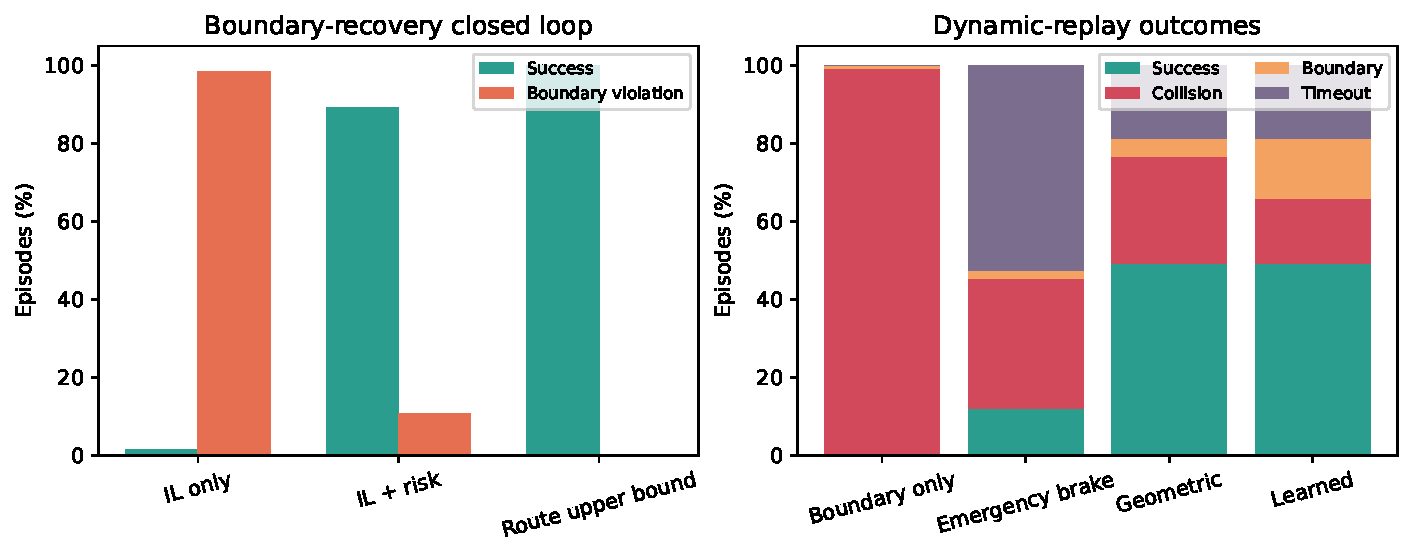
\includegraphics[width=0.92\textwidth]{figures/closed_loop_results.pdf}
\caption{Closed-loop outcomes on M0S7. Left: boundary recovery over 130 episodes. Right: outcomes for 150 controlled dynamic-replay interactions.}
\label{fig:closed_loop_results}
\end{figure*}

\subsection{Statistical Scope and Limitations}
\label{sec:statistics}

The boundary-recovery methods are evaluated on the same 130 initial conditions, and the dynamic-replay methods use the same 150 interactions, enabling paired comparisons within each experiment. The collision-risk model is trained with three random seeds, whereas the imitation and boundary-risk models currently use one seed. Consequently, only collision-prediction variance is reported explicitly, and the closed-loop results should be interpreted as controlled paired comparisons rather than a complete statistical evaluation. Individual frames, augmented candidate pairs, and replay episodes derived from the same source track are not treated as independent real-world trials.

The M0S7 geometry is available to the simulator for rendering observations and defining the controlled evaluation corridor, while its trajectory samples and outcomes are excluded from training and model selection. The dynamic test uses only five source tracks and augments their relative placement and timing; augmented episodes are not independent real encounters. The reported setting therefore measures known-geometry, held-out-traversal performance. It does not demonstrate operation in an unmapped mine, cross-mine transfer, long-term environmental change, high-fidelity vehicle dynamics, or physical-platform safety.
